\documentclass[11pt,a4paper]{article}
\usepackage{fontspec}
\setmainfont{TeX Gyre Pagella}
\newfontfamily\headfont{Inter}[UprightFont=*-ExtraBold,BoldFont=*-ExtraBold,Extension=.otf,Path=/usr/share/fonts/opentype/inter/]
\usepackage[a4paper,margin=2.3cm]{geometry}
\usepackage{graphicx,booktabs,float,caption,array,xcolor,longtable}
\usepackage{xurl}
\usepackage[hidelinks]{hyperref}
\usepackage{titlesec}
\usepackage[round]{natbib}
\usepackage{setspace}
\setstretch{1.05}
\renewcommand{\topfraction}{0.9}
\renewcommand{\bottomfraction}{0.8}
\renewcommand{\textfraction}{0.1}
\renewcommand{\floatpagefraction}{0.75}
\setlength{\parindent}{0pt}
\setlength{\parskip}{0.55em}
\titleformat{\section}{\headfont\Large}{\thesection}{0.8em}{}
\titleformat{\subsection}{\headfont\large}{\thesubsection}{0.8em}{}
\captionsetup{font=small,labelfont=bf}
\urlstyle{same}
\hypersetup{pdftitle={Waterloo Road and the Clock in the Streets},pdfauthor={Tristan Hotham}}

\begin{document}
\begin{center}
{\Large\bfseries Waterloo Road and the Clock in the Streets\par}
\vspace{0.4em}
{\large Battle street names and the growth of British towns, from OpenStreetMap\par}
\vspace{1.2em}
{\large Tristan Hotham\par}
\vspace{0.3em}
{\small Independent researcher\\
ORCID: 0000-0003-4931-9349\\
DOI: https://doi.org/10.5281/zenodo.24086515\par}
\vspace{0.8em}
2026
\end{center}

\begin{quote}
\small
\begin{center}\textbf{Abstract}\end{center}
Nineteenth-century builders often named new streets after recent victories, so battle names may record when a street was laid out. I match 6,885 OpenStreetMap highways in the United Kingdom against a table of 111 battles, join the pieces of each street into 3,352 streets, and set aside streets named after battles before 1793 (1,008) and names that usually refer to something else (654: Nile, Quebec, Kimberley and others). Of 1,690 streets named after 54 battles from 1793 to 1944, Waterloo (367), Alma (340) and Trafalgar (241) lead; the four Crimean battles gave 425 streets, more than both world wars together (315), and world-war names are much more often modern estate names (39.4\% Close, Drive, Way and the like, against 12.9\% for 1854 to 1902). Within towns, streets named after later battles lie farther from the centre: the mean within-town Spearman correlation of battle date and distance is 0.25 across 75 towns (53 positive, 19 negative; permutation $p<0.001$, or $p<0.01$ with clusters of same-war streets counted once). Ranked within their towns, Napoleonic streets sit at 0.54, Crimean at 0.58 and Boer War streets at 0.68 of the way from centre to edge. The clock is real but coarse: it separates wars half a century apart, not neighbouring ones.

\textbf{Keywords:} street names; commemoration; urban growth; toponymy; battles; OpenStreetMap
\end{quote}

\section{Introduction}
Street names are a public record of what a society chose to commemorate \citep{azaryahu1996,alderman2000,roseredwood2010}. In Victorian Britain one common choice was the latest victory: Alma Road and Inkerman Street after 1854, Ladysmith Road and Mafeking Street in 1900. If developers named streets as they were laid out, and if towns grew outwards, battle names should form a crude clock in the street plan, with older victories near the centre and newer ones farther out, echoing the rings of growth that urban morphologists have traced in British towns \citep{conzen1960,whitehand1972}. This paper asks whether the clock is there, using an open map of every street in the United Kingdom.

\section{Data}
\textbf{Streets.} OpenStreetMap ways with a \texttt{highway} tag in the United Kingdom whose names contain a battle name, queried with QLever \citep{bast2017}: 6,885 ways with highway type, name and first coordinate. OpenStreetMap's coverage of names is good in towns but uneven \citep{haklay2010}. \textbf{Towns.} Wikidata settlements typed as towns or cities with a population (CC0). \textbf{Counties.} ONS boundaries.

\textbf{Battle table.} Each battle has the date of the battle, or for a siege the date of its relief or fall (Table~\ref{tab:battles}). Battles before 1793 are kept but set aside from the clock, since a street named Naseby or Agincourt was named centuries after the event. Names that usually refer to a place, a person or a colour are flagged as ambiguous and set aside: Aboukir, Alexandria, Cabul, Copenhagen, Crimea, Delhi, Dunkirk, Falklands, Gibraltar, Kandahar, Kimberley, Magenta, Minorca, Nile, Portobello, Quebec, Scinde, St Vincent and Vigo. The Nile, for example, is far more often the river; London's Copenhagen Street takes its name from the area around Copenhagen House, a seventeenth-century house far older than the battle; Dunkirk was an English place name long before 1940; Magenta is a colour, itself named after the battle.

\section{Method}
\textbf{Matching and joining.} Names were matched to the battle table as whole words; names of twin towns (Villiers-sur-Marne Avenue) were excluded. Pieces with the same normalised name were joined when their first points chain within 600 m, and pieces of through roads (primary to unclassified, tracks, cycle paths) within 1.5 km, which joined 3,509 pieces into others; 11 pairs of same-named streets within 1.5 km remain separate, since they may be distinct streets. The full list of names for each battle was read; 9 were removed by hand (\texttt{code/overrides.csv}): non-streets such as pothole markers, moorings and railway sidings, Alma Martin Way, De-Verdun Avenue, and Arras Hill near Market Weighton, an old Yorkshire place name. 32 streets named after battles from 1793 on lie within 3 km of a Wikidata place containing the battle's name (Waterloo in London and on Merseyside, Inkerman in County Durham, Camperdown in Dundee) and are set aside as probably named after the place.

\textbf{Towns and distance.} Each street is assigned to the nearest town of at least 20,000 people within 10 km, with all of Greater London counted as London, and its distance from the town's Wikidata point is measured. \textbf{Street words.} The last word of the name is classed as traditional (Street, Road, Terrace, Place, Row, Square, Grove, Crescent, Lane, Villas and similar), modern (Close, Drive, Way, Court, Mews, Rise, View, Gardens and similar) or other.

\textbf{The clock test.} The main test uses streets named after battles from 1793 on, with a traditional street word, not ambiguous or place-named, in a town. For each town with at least four such streets and two distinct battle years, I compute Spearman's rank correlation between battle year and distance from the centre. The statistic is the mean correlation across towns; its null distribution comes from 4,000 permutations of battle years within towns, which keeps each town's set of distances and dates. A sign test on the number of positive and negative towns is reported alongside. As a second view, each street's distance is ranked within its town (towns with three or more streets) and the mean rank percentile is computed for each war with a bootstrap interval; with no clock every war would sit at 0.5.

\begin{small}\begin{longtable}{llp{5.2cm}lr}\caption{The battles found in street names: date used, war, status (old: before 1793, set aside; amb.: ambiguous name, set aside) and number of streets.}\label{tab:battles}\\\toprule Battle & Date & War & Status & Streets\\\midrule\endhead
Armada & 1588-08-08 & Spanish Armada & old & 28\\
Bannockburn & 1314-06-24 & Scottish independence & old & 12\\
Crecy & 1346-08-26 & Hundred Years War & old & 14\\
Poitiers & 1356-09-19 & Hundred Years War & old & 2\\
Agincourt & 1415-10-25 & Hundred Years War & old & 27\\
Bosworth & 1485-08-22 & Wars of the Roses & old & 73\\
Flodden & 1513-09-09 & Anglo-Scottish wars & old & 9\\
Edgehill & 1642-10-23 & English Civil War & old & 68\\
Marston Moor & 1644-07-02 & English Civil War & old & 5\\
Naseby & 1645-06-14 & English Civil War & old & 78\\
Sedgemoor & 1685-07-06 & Monmouth Rebellion & old & 40\\
Boyne & 1690-07-11 & Williamite War & old & 31\\
Aughrim & 1691-07-22 & Williamite War & old & 10\\
Vigo & 1702-10-23 & Spanish Succession & amb. & 22\\
Blenheim & 1704-08-13 & Spanish Succession & old & 478\\
Gibraltar & 1704-08-04 & Spanish Succession & amb. & 52\\
Ramillies & 1706-05-23 & Spanish Succession & old & 19\\
Almanza & 1707-04-25 & Spanish Succession & old & 1\\
Oudenarde & 1708-07-11 & Spanish Succession & old & 1\\
Malplaquet & 1709-09-11 & Spanish Succession & old & 1\\
Portobello & 1739-11-22 & Jenkins' Ear & amb. & 32\\
Dettingen & 1743-06-27 & Austrian Succession & old & 6\\
Fontenoy & 1745-05-11 & Austrian Succession & old & 2\\
Culloden & 1746-04-16 & Jacobite rising & old & 28\\
Minorca & 1756-05-20 & Seven Years War & amb. & 16\\
Plassey & 1757-06-23 & Seven Years War & old & 11\\
Louisburg & 1758-07-26 & Seven Years War & old & 1\\
Minden & 1759-08-01 & Seven Years War & old & 34\\
Quebec & 1759-09-13 & Seven Years War & amb. & 72\\
Quiberon & 1759-11-20 & Seven Years War & old & 1\\
Belle Isle & 1761-06-07 & Seven Years War & old & 15\\
Havannah & 1762-08-13 & Seven Years War & old & 13\\
St Vincent & 1797-02-14 & French Revolutionary Wars & amb. & 59\\
Camperdown & 1797-10-11 & French Revolutionary Wars &  & 27\\
Nile & 1798-08-01 & French Revolutionary Wars & amb. & 54\\
Aboukir & 1798-08-01 & French Revolutionary Wars & amb. & 2\\
Copenhagen & 1801-04-02 & French Revolutionary Wars & amb. & 22\\
Alexandria & 1801-03-21 & French Revolutionary Wars & amb. & 24\\
Trafalgar & 1805-10-21 & Napoleonic Wars &  & 241\\
Maida & 1806-07-04 & Napoleonic Wars &  & 23\\
Vimeiro & 1808-08-21 & Peninsular War &  & 1\\
Corunna & 1809-01-16 & Peninsular War &  & 21\\
Talavera & 1809-07-28 & Peninsular War &  & 11\\
Salamanca & 1812-07-22 & Peninsular War &  & 14\\
Vittoria & 1813-06-21 & Peninsular War &  & 8\\
Waterloo & 1815-06-18 & Napoleonic Wars &  & 367\\
Algiers & 1816-08-27 & Bombardment of Algiers &  & 4\\
Navarino & 1827-10-20 & Greek War of Independence &  & 4\\
Cabul & 1842-09-15 & First Anglo-Afghan War & amb. & 3\\
Meeanee & 1843-02-17 & Conquest of Sind &  & 2\\
Scinde & 1843-02-17 & Conquest of Sind & amb. & 1\\
Moodkee & 1845-12-18 & First Anglo-Sikh War &  & 1\\
Ferozeshah & 1845-12-21 & First Anglo-Sikh War &  & 1\\
Aliwal & 1846-01-28 & First Anglo-Sikh War &  & 3\\
Sobraon & 1846-02-10 & First Anglo-Sikh War &  & 2\\
Goojerat & 1849-02-21 & Second Anglo-Sikh War &  & 1\\
Alma & 1854-09-20 & Crimean War &  & 340\\
Balaclava & 1854-10-25 & Crimean War &  & 22\\
Inkerman & 1854-11-05 & Crimean War &  & 57\\
Sebastopol & 1855-09-09 & Crimean War &  & 6\\
Crimea & 1855-09-09 & Crimean War & amb. & 14\\
Delhi & 1857-09-20 & Indian Rebellion & amb. & 18\\
Cawnpore & 1857-07-16 & Indian Rebellion &  & 5\\
Lucknow & 1857-11-16 & Indian Rebellion &  & 21\\
Magenta & 1859-06-04 & Second Italian War & amb. & 11\\
Ulundi & 1879-07-04 & Anglo-Zulu War &  & 3\\
Kandahar & 1880-09-01 & Second Anglo-Afghan War & amb. & 4\\
Majuba & 1881-02-27 & First Boer War &  & 3\\
Tel el Kebir & 1882-09-13 & Anglo-Egyptian War &  & 1\\
Khartoum & 1885-01-26 & Mahdist War &  & 14\\
Dargai & 1897-10-20 & Tirah Campaign &  & 3\\
Omdurman & 1898-09-02 & Mahdist War &  & 2\\
Modder River & 1899-11-28 & Second Boer War &  & 5\\
Colenso & 1899-12-15 & Second Boer War &  & 33\\
Spion Kop & 1900-01-24 & Second Boer War &  & 9\\
Kimberley & 1900-02-15 & Second Boer War & amb. & 173\\
Tugela & 1900-02-27 & Second Boer War &  & 4\\
Ladysmith & 1900-02-28 & Second Boer War &  & 73\\
Mafeking & 1900-05-17 & Second Boer War &  & 43\\
Mons & 1914-08-23 & First World War &  & 30\\
Marne & 1914-09-06 & First World War &  & 30\\
Ypres & 1914-10-19 & First World War &  & 13\\
Gallipoli & 1915-04-25 & First World War &  & 5\\
Anzac & 1915-04-25 & First World War &  & 7\\
Verdun & 1916-02-21 & First World War &  & 18\\
Jutland & 1916-05-31 & First World War &  & 34\\
Somme & 1916-07-01 & First World War &  & 12\\
Arras & 1917-04-09 & First World War &  & 18\\
Vimy & 1917-04-09 & First World War &  & 12\\
Messines & 1917-06-07 & First World War &  & 6\\
Cambrai & 1917-11-20 & First World War &  & 21\\
Dunkirk & 1940-05-26 & Second World War & amb. & 55\\
Tobruk & 1941-04-10 & Second World War &  & 9\\
Alamein & 1942-10-23 & Second World War &  & 35\\
Anzio & 1944-01-22 & Second World War &  & 12\\
Cassino & 1944-01-17 & Second World War &  & 7\\
Kohima & 1944-04-04 & Second World War &  & 8\\
Imphal & 1944-03-08 & Second World War &  & 1\\
Arnhem & 1944-09-17 & Second World War &  & 37\\
Falklands & 1982-04-02 & Falklands War & amb. & 20\\
\bottomrule\end{longtable}\end{small}

\section{Results}
\subsection{Which battles}
The 1,690 streets after battles from 1793 on are dominated by three names: Waterloo (367), Alma (340) and Trafalgar (241), followed by Ladysmith (73), Inkerman (57) and Mafeking (43) (Figure~\ref{fig:bursts}). Before 1793, Blenheim is the commonest battle name of all (478), though often through Blenheim Palace. The names come in bursts: after Waterloo the battles of 1816 to 1853 gave only 18 streets, while the Crimean War gave 425 in two years. The First World War gave 206 and the Second 109. By county, Greater London (126), Greater Manchester (91) and West Yorkshire (82) have the most; the Alma is the commonest battle in 18 of 46 English counties, and Trafalgar leads in naval Hampshire and Devon (Figure~\ref{fig:map}).

\begin{figure}[tbp]\centering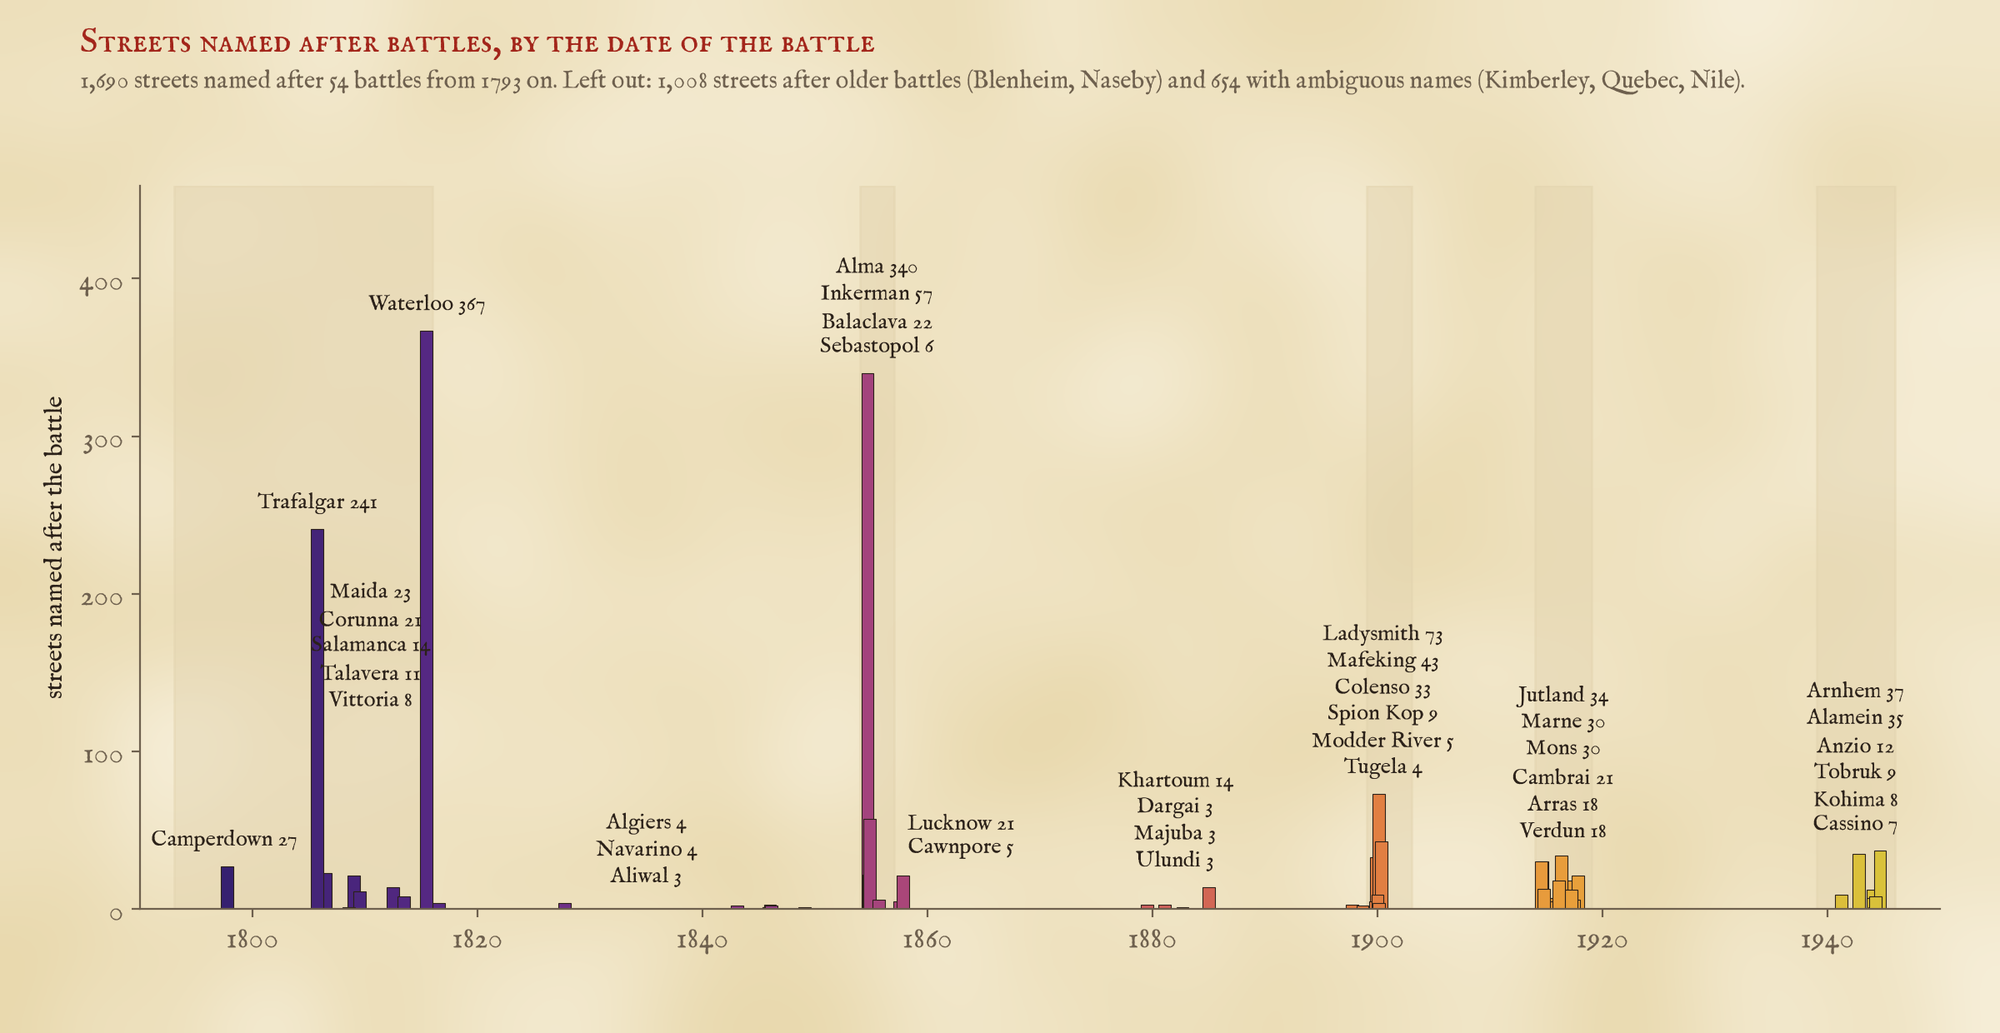
\includegraphics[width=\textwidth]{f_bursts.png}
\caption{Streets named after each battle from 1793 on, by the date of the battle.}\label{fig:bursts}\end{figure}

\begin{figure}[tbp]\centering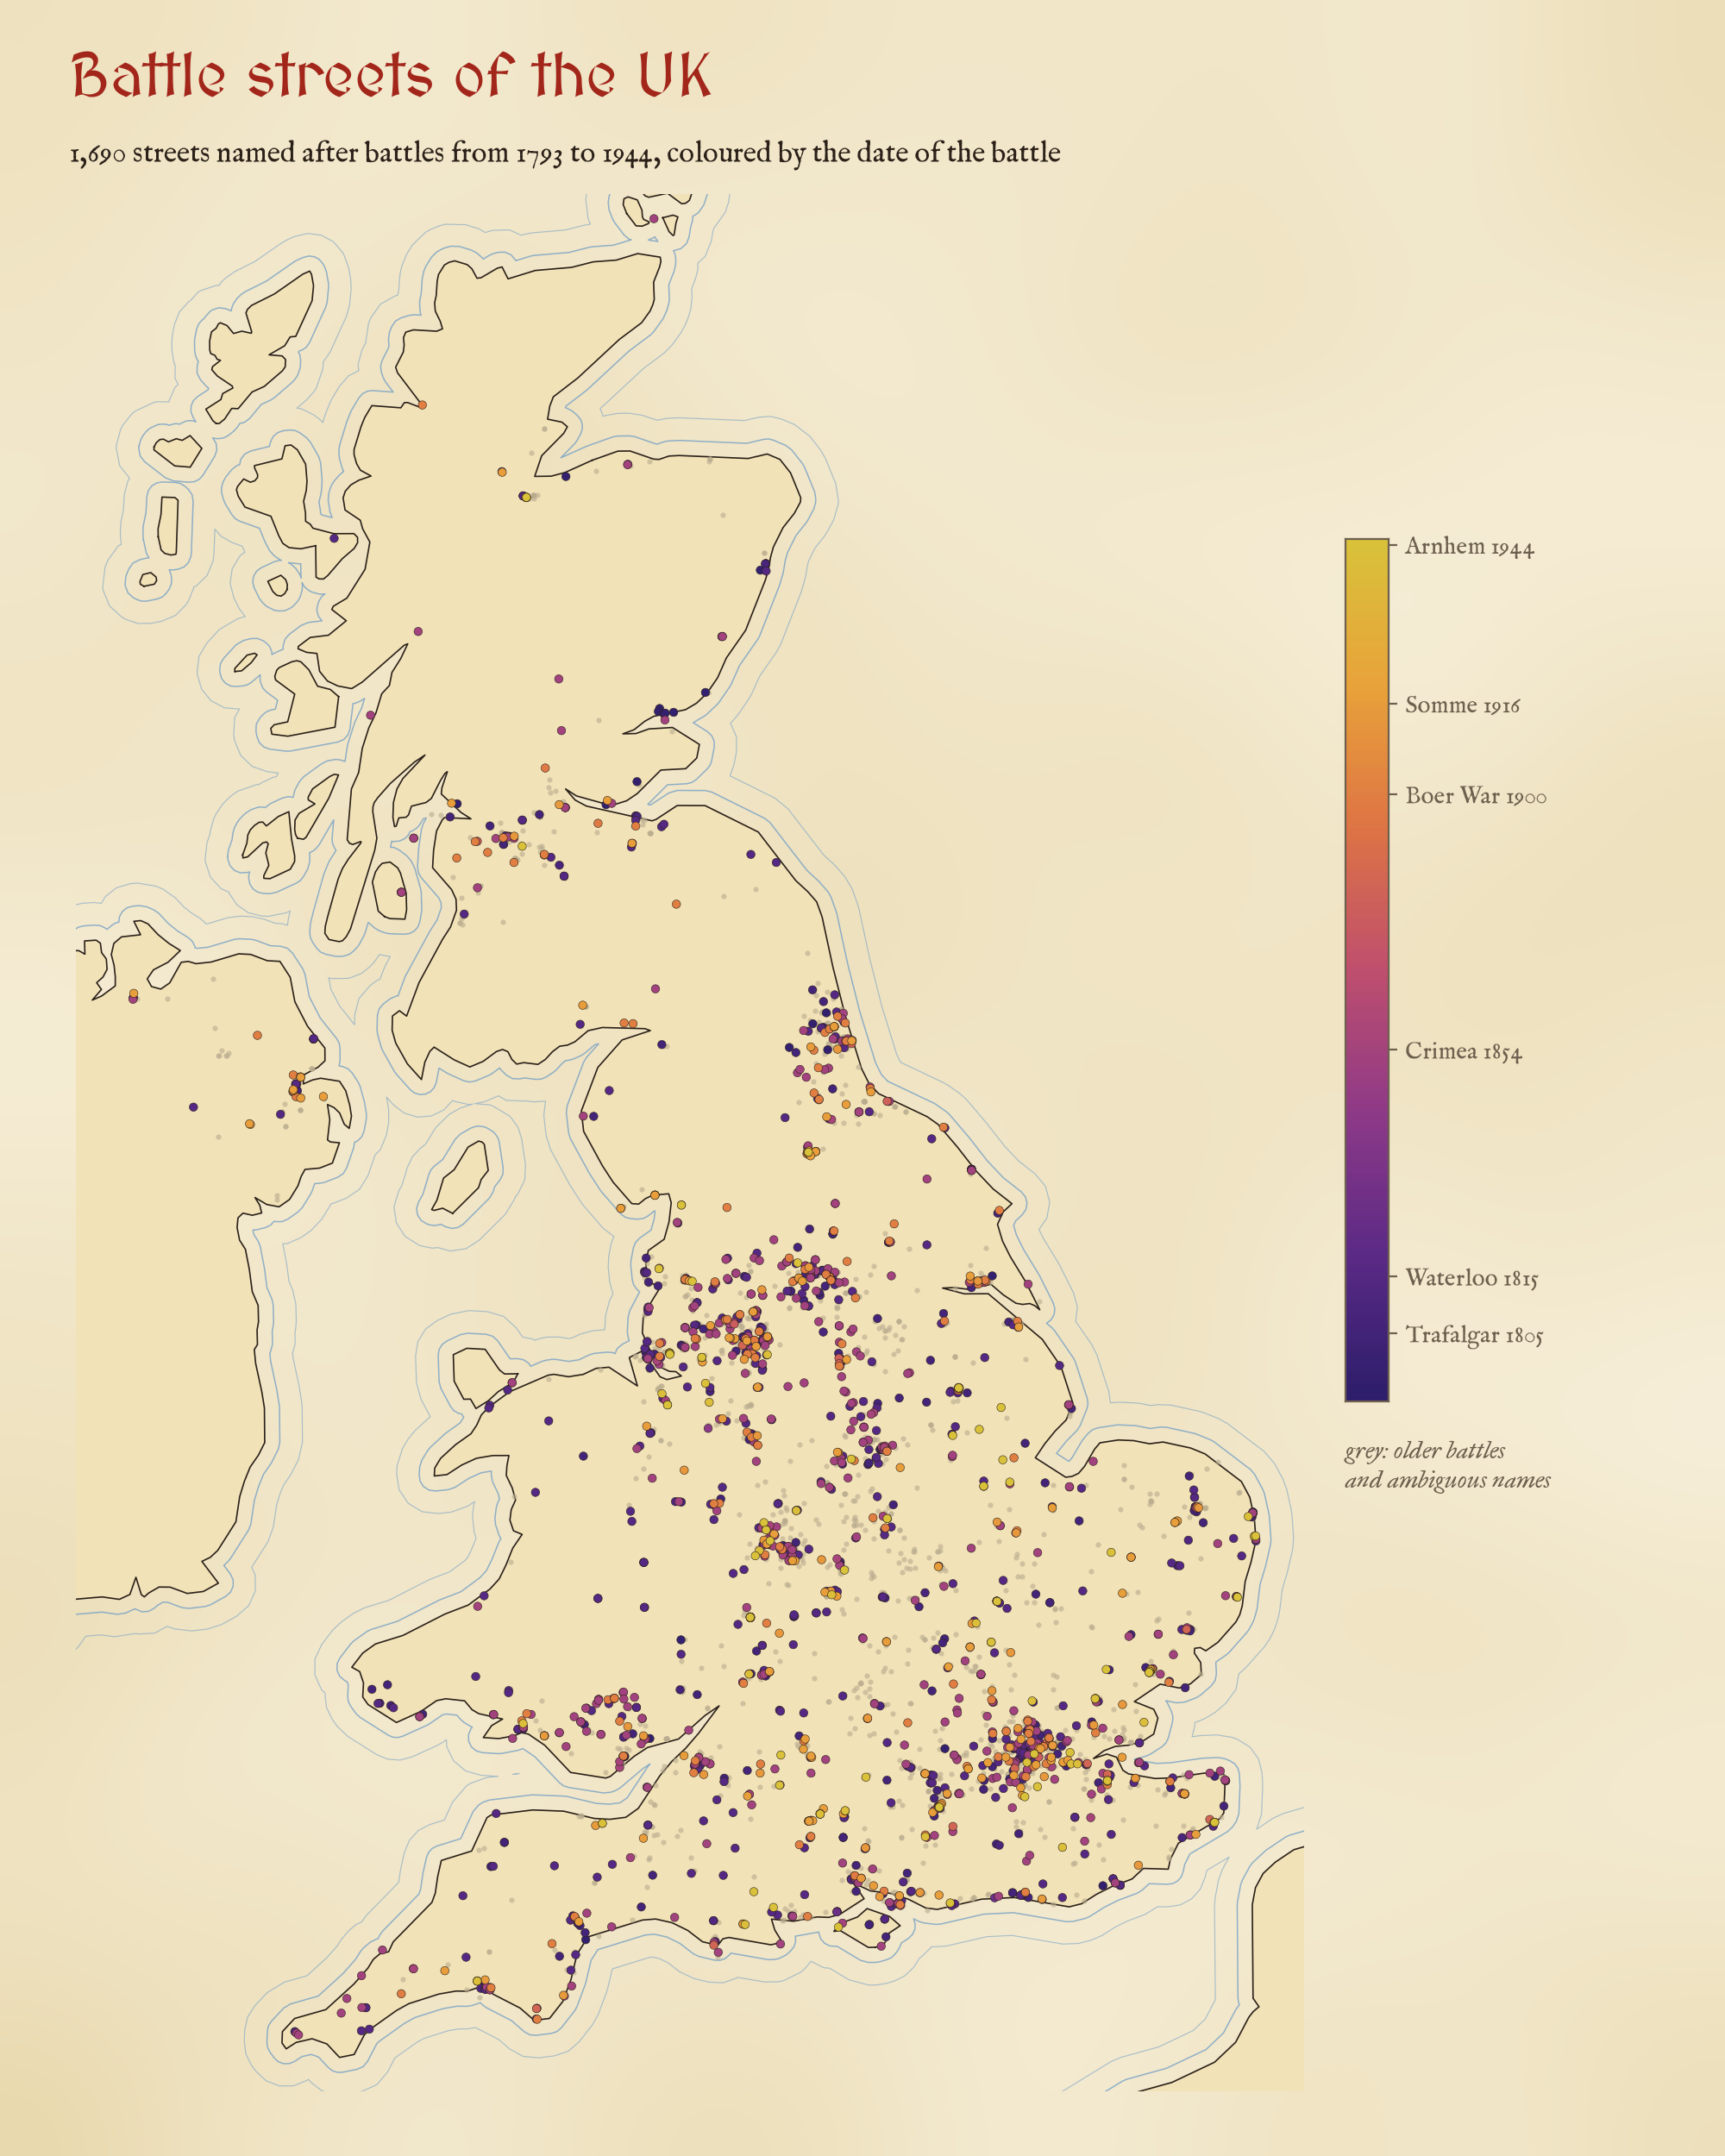
\includegraphics[width=0.8\textwidth]{f_map.png}
\caption{Battle streets in the United Kingdom, coloured by the date of the battle; grey: older battles and ambiguous names.}\label{fig:map}\end{figure}

\subsection{Named at the time, or later?}
For battles from 1854 to 1902, 78.9\% of streets end in a traditional word and 12.9\% in a modern one. For the world-war battles the modern share is 39.4\% (Figure~\ref{fig:style}), consistent with many of those names being chosen as estate themes decades after the war. Waterloo and Trafalgar also kept being reused: 33.2\% of Trafalgar streets and 19.9\% of Waterloo streets have a modern street word. This is why the main test uses traditional street words only.

\begin{figure}[tbp]\centering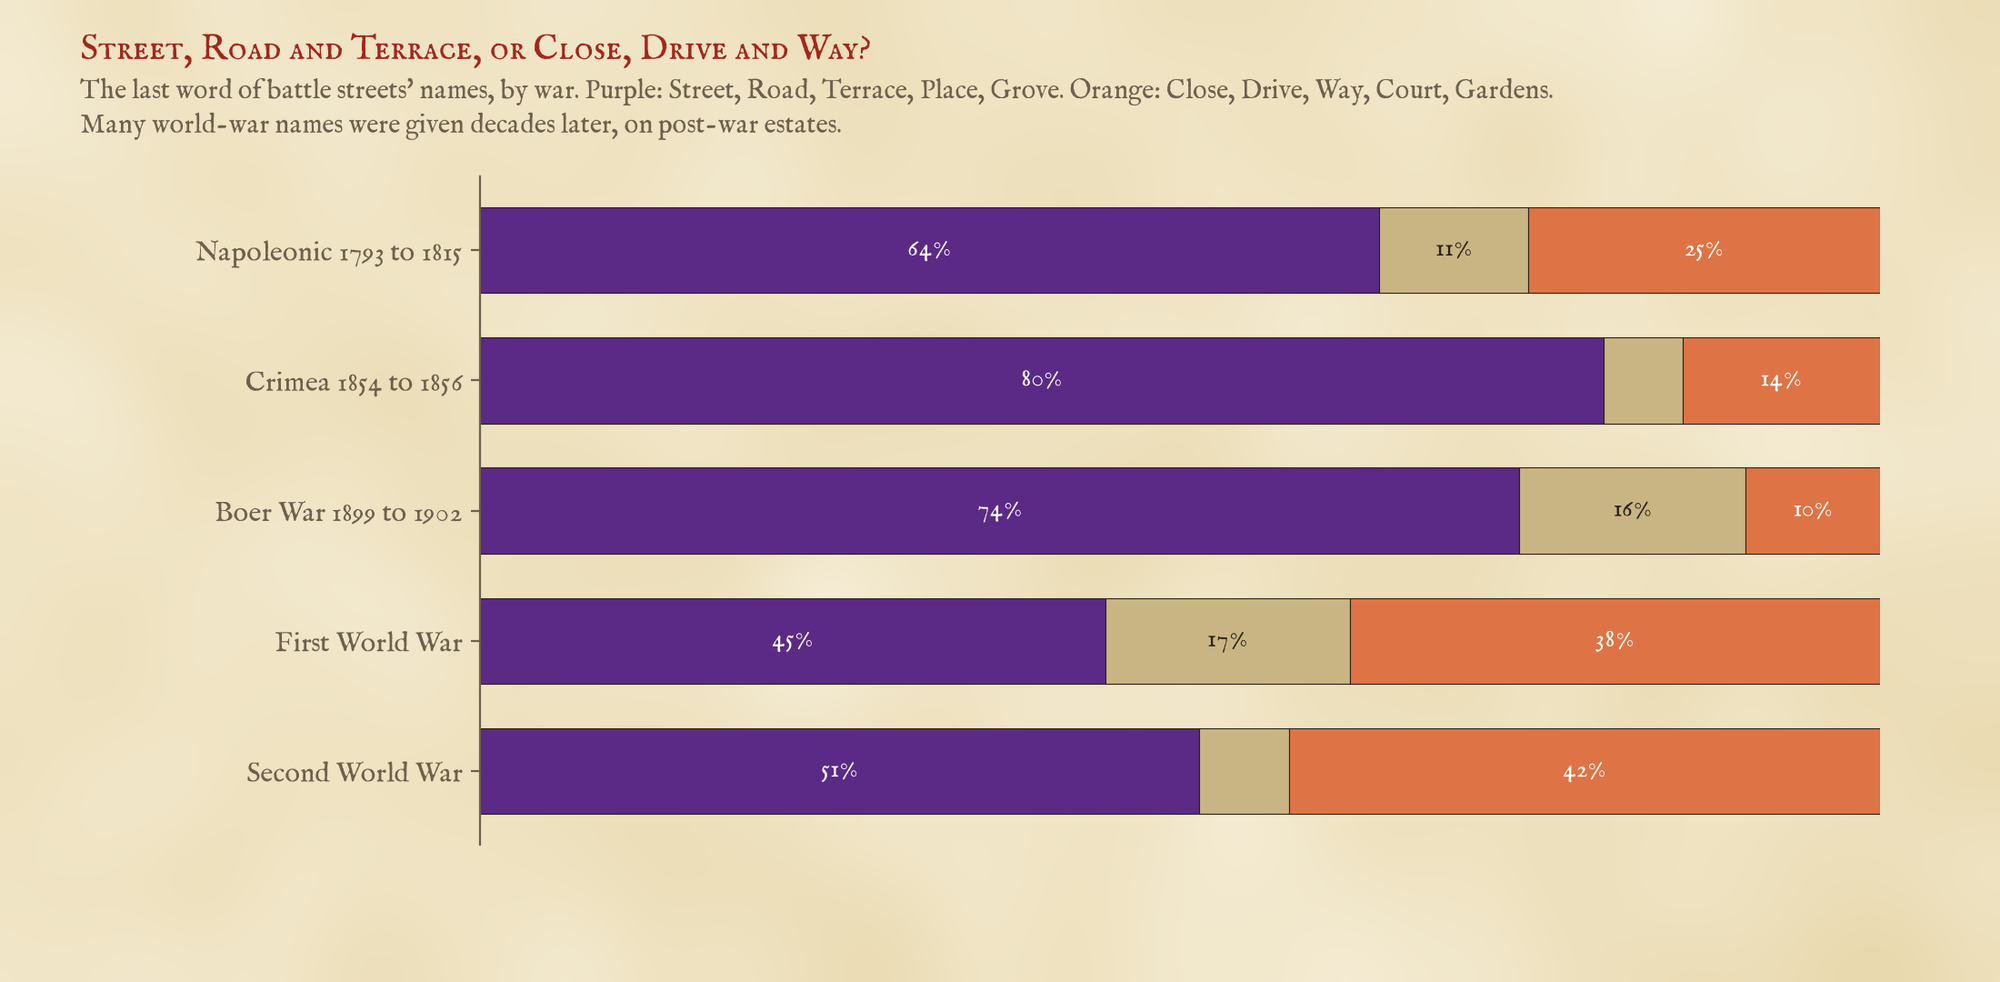
\includegraphics[width=0.92\textwidth]{f_style.png}
\caption{The last word of battle street names, by war.}\label{fig:style}\end{figure}

\subsection{The clock}
Across 75 towns with four or more streets (549 streets), the mean within-town correlation of battle year and distance is 0.25 (median 0.32); 53 towns are positive and 19 negative (sign test $p=0.00004$). None of 4,000 within-town permutations reached the observed mean; the 97.5th percentile of the null is 0.11 (Figure~\ref{fig:clock}). The result holds without London (mean 0.26, 74 towns), for towns with six or more streets (0.25, 36 towns), and for battles up to 1902 only (0.18, 62 towns, 4 of 4,000 permutations as high). With all street words it is weaker (0.14, 110 towns, 6 of 4,000 permutations as high), as expected if modern names were given late. The permutation test treats streets as independent, but streets of one war often stand together and were probably named together. Counting each cluster of same-war streets within 500 m of each other in a town as one unit (792 units), the mean correlation falls to 0.16 across 51 towns (32 positive, 17 negative), with 27 of 4,000 permutations as high ($p=0.007$). The clock survives, but the street-level test overstates its precision.

\begin{figure}[tbp]\centering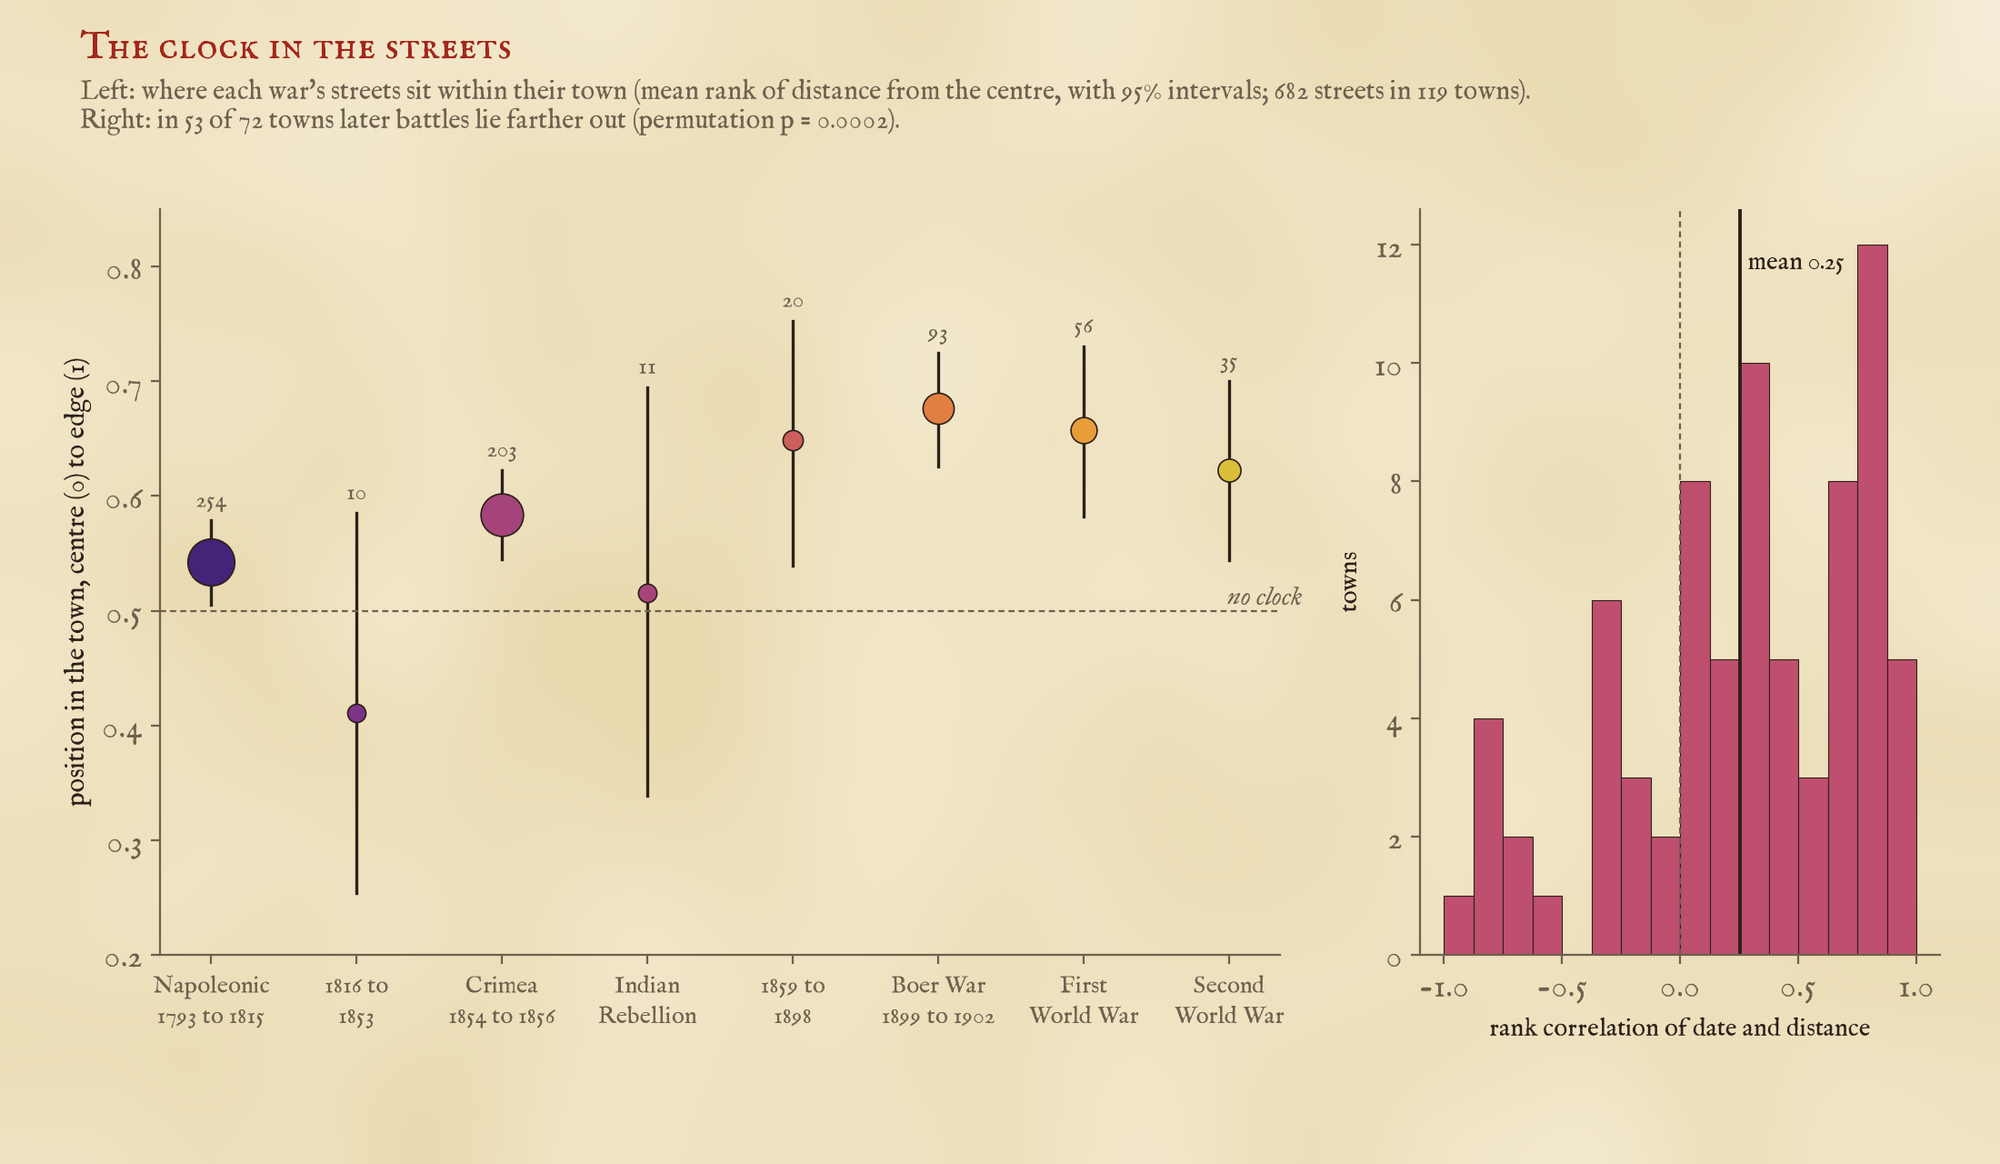
\includegraphics[width=\textwidth]{f_clock.png}
\caption{Left: mean within-town rank of distance by war, with 95\% bootstrap intervals. Right: within-town correlations of battle date and distance.}\label{fig:clock}\end{figure}

Within their towns, Napoleonic streets sit at a mean rank of 0.54 (interval 0.51 to 0.58), Crimean at 0.58 (0.54 to 0.62), Boer War at 0.68 (0.63 to 0.72) and First World War at 0.66; median distances are 1.45, 2.01, 2.36 and 3.00 km.

\subsection{A coarse clock}
Pairwise, the clock separates wars far apart but not neighbours. Napoleonic streets are nearer the centre than Boer War streets in 30 of 40 towns with both, Crimean than Boer War in 23 of 38, but Napoleonic than Crimean in only 47 of 92, and Boer War than First World War in 8 of 17. Individual towns vary (Figure~\ref{fig:towns}): Bristol (0.66), Glasgow (0.75) and Hull (0.84) keep good time, London barely (0.12), and Preston (-0.33) and Lincoln (-0.84) run backwards.

\begin{figure}[tbp]\centering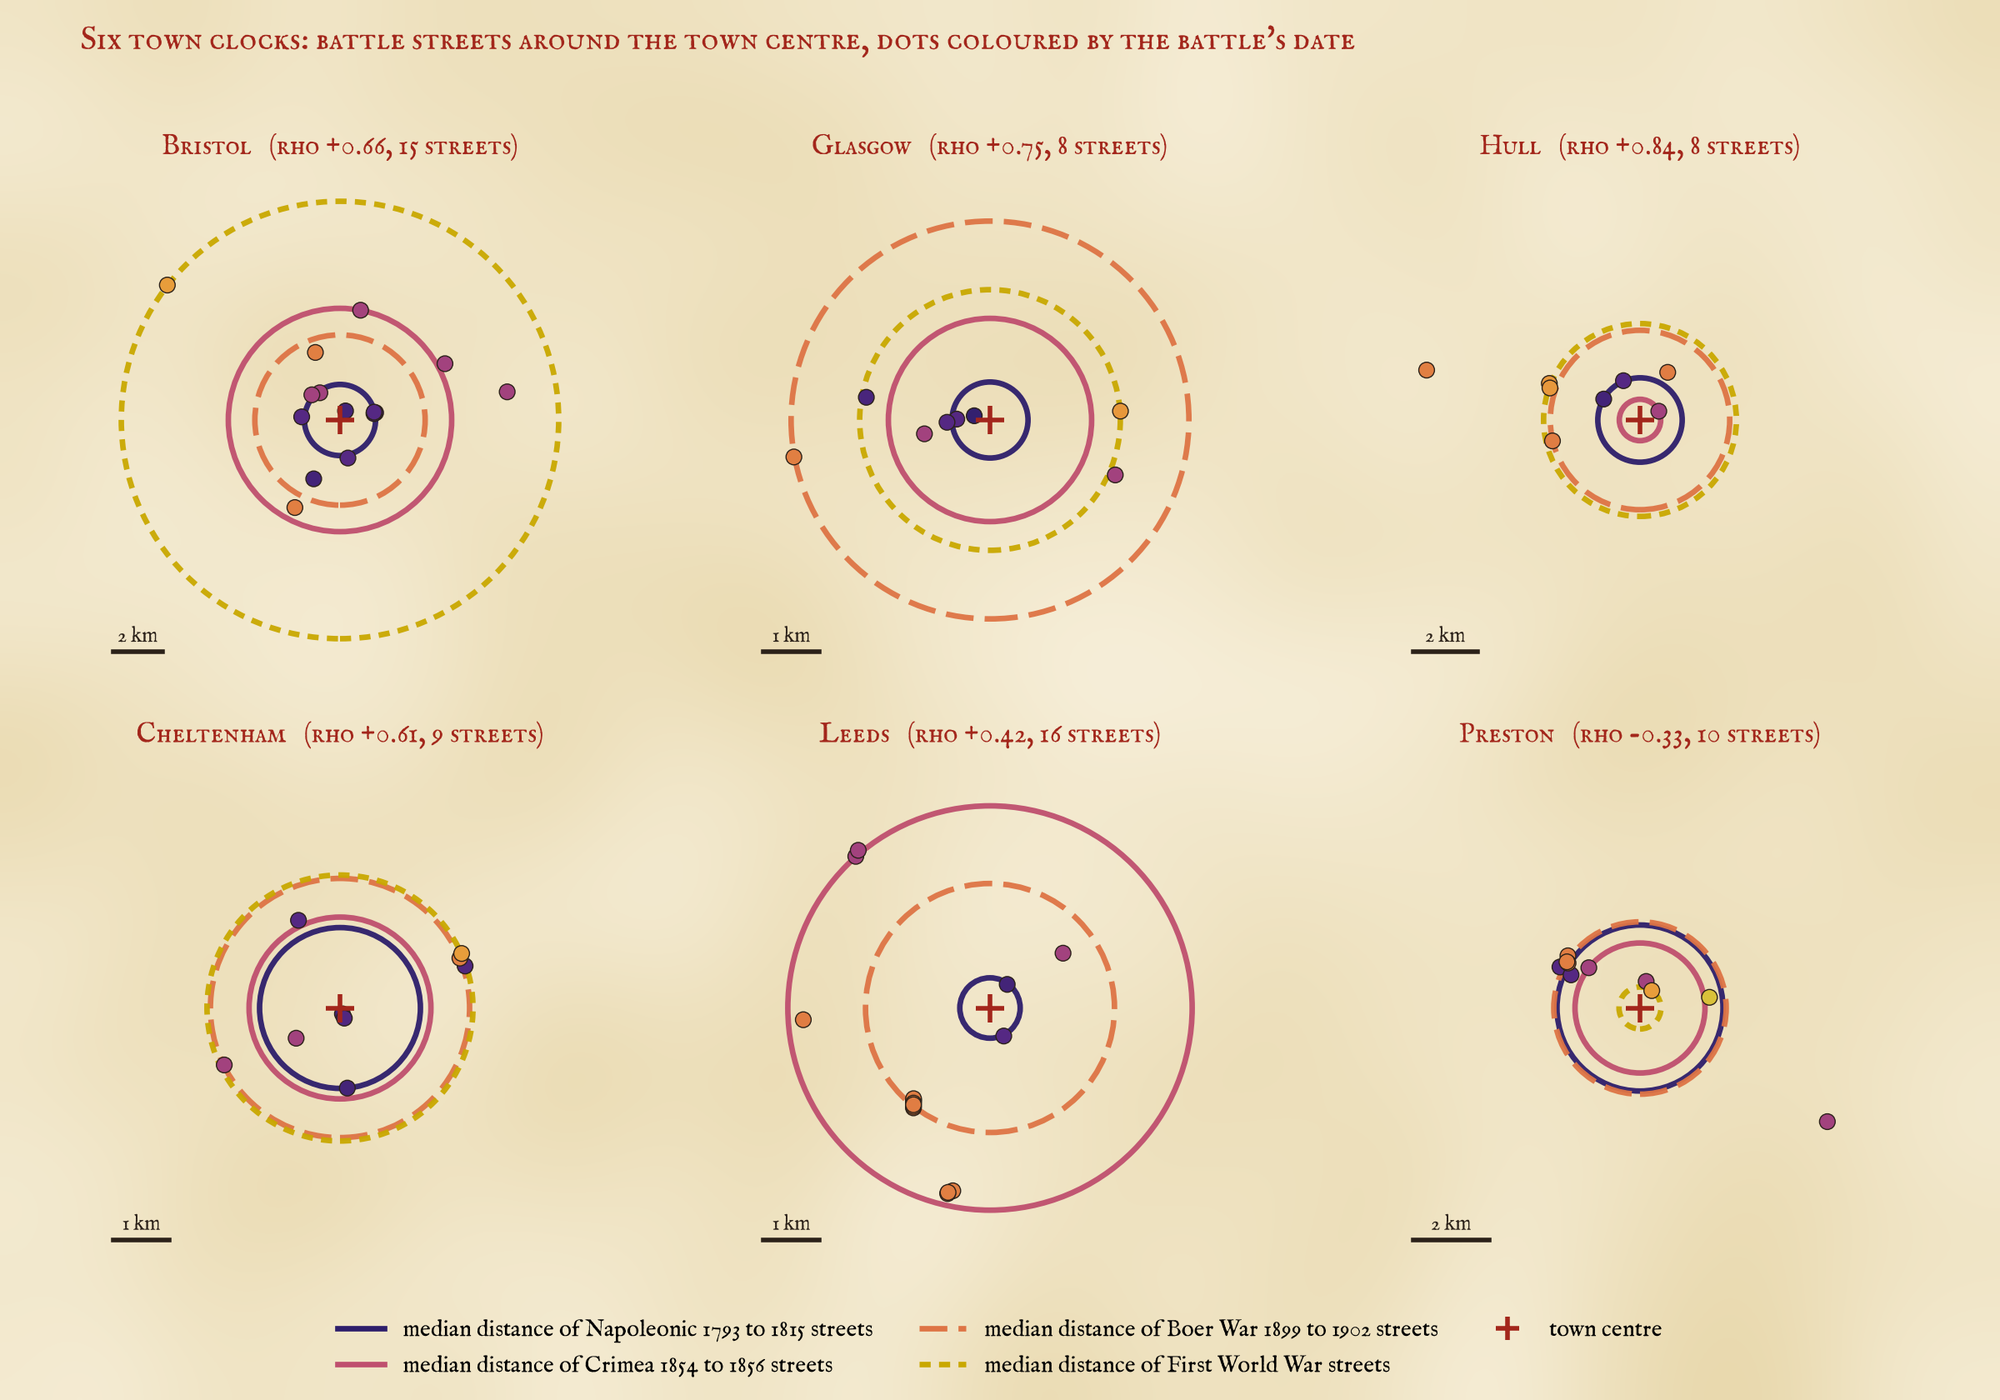
\includegraphics[width=\textwidth]{f_towns.png}
\caption{Six towns: battle streets around the centre and the median distance of each war's streets.}\label{fig:towns}\end{figure}

\section{Limitations}
The name dates the battle, not the street: some streets were named long after their battle, some renamed, and Waterloo and Trafalgar especially stayed in fashion. The traditional street-word filter reduces but does not remove late naming. Towns did not grow in rings: they grew along roads and railways and around industry, and a conurbation's streets are assigned to whichever town point is nearest, which compresses distances. Town centres are Wikidata points. Alma is also a woman's name: 70 of the 340 Alma streets lack a traditional street word, and 50 of these lie more than 1 km from any traditional Alma street, so some may commemorate a person or a house; even if all 50 were removed, the Crimean battles would give 375 streets, still more than both world wars. These streets are outside the main test, which uses traditional street words only. The ambiguity and place-name rules are judgements, documented in the code; a few ambiguous names may be battles and a few kept names may not be. Each street is placed at the mean of the first points of its pieces. OpenStreetMap names are incomplete in places, and the counts for many battles are small.

\section{Conclusion}
Battle names do carry a clock. Across British towns, streets named after later battles lie farther from the centre, clearly enough that no shuffle of the dates matched it, though counting clusters of same-war streets once makes the signal weaker. But it is a slow clock that runs fast in places: it tells the French wars from the Boer War, not Waterloo from the Alma. The bursts of names, the Crimea above all, and the shift of world-war names onto post-war estates are as telling as the rings.

\section*{Data and code availability}
The interactive map is at \url{https://maps.tristanhotham.com/battle-streets/}. Code, the battle table, the rules and hand decisions, and the derived tables are at \url{https://github.com/Tristan-Hotham/battle-streets} and archived with this paper at https://doi.org/10.5281/zenodo.24086515. The street tables are derived from OpenStreetMap (\copyright{} OpenStreetMap contributors) and released under the Open Database Licence; Wikidata is CC0; county boundaries from the ONS (Open Government Licence v3.0); text and figures CC BY 4.0; code MIT.

\section*{AI statement}
I wrote the text, with drafting and editing assistance from Claude (Anthropic), which also helped prepare the analysis code. I reviewed and checked all text and results.

\begin{thebibliography}{10}
\bibitem[Alderman(2000)]{alderman2000} Alderman, D. H. (2000) A street fit for a King: naming places and commemoration in the American South. \textit{The Professional Geographer} 52(4), 672 to 684.
\bibitem[Azaryahu(1996)]{azaryahu1996} Azaryahu, M. (1996) The power of commemorative street names. \textit{Environment and Planning D: Society and Space} 14(3), 311 to 330.
\bibitem[Bast and Buchhold(2017)]{bast2017} Bast, H. and Buchhold, B. (2017) QLever: a query engine for efficient SPARQL+Text search. \textit{Proceedings of the 2017 ACM Conference on Information and Knowledge Management (CIKM)}, 647 to 656.
\bibitem[Conzen(1960)]{conzen1960} Conzen, M. R. G. (1960) \textit{Alnwick, Northumberland: A Study in Town-Plan Analysis}. Institute of British Geographers Publication 27. London: George Philip.
\bibitem[Haklay(2010)]{haklay2010} Haklay, M. (2010) How good is volunteered geographical information? A comparative study of OpenStreetMap and Ordnance Survey datasets. \textit{Environment and Planning B: Planning and Design} 37(4), 682 to 703.
\bibitem[Rose-Redwood et al.(2010)]{roseredwood2010} Rose-Redwood, R., Alderman, D. and Azaryahu, M. (2010) Geographies of toponymic inscription: new directions in critical place-name studies. \textit{Progress in Human Geography} 34(4), 453 to 470.
\bibitem[Whitehand(1972)]{whitehand1972} Whitehand, J. W. R. (1972) Building cycles and the spatial pattern of urban growth. \textit{Transactions of the Institute of British Geographers} 56, 39 to 55.
\end{thebibliography}
\end{document}
